\chapter{Einführung}

Diese Einführung dient als Wegweiser durch die vorliegende Arbeit und soll einen kurzen Überblick über die folgenden Kapitel und deren Inhalt geben.

\section{Überblick}

In \fref{chap:engine-uebersicht} wird mit einer Übersicht über die aktuellen Strömungen der Spiele- und Grafik-Engine-Entwicklung begonnen. Das Kapitel wird aufzeigen, dass Spieleengines komplexe, dynamische und interdisziplinäre Softwareprojekte sind. Die unterschiedlichen Engines teilen einige gemeinsame Anforderungen und Herausforderungen. Das Kapitel wird einige der gemeinsamen Herausforderungen aufzeigen, von denen sich viele auch auf Projekte aus anderen Branchen übertragen lassen.

Abseits der Komplexität von Spiele-Engines gibt es seit wenigen Jahren Bestrebungen die bestehenden, über die Jahre gewachsenen, Grafikschnittstellen wie \textit{DirectX} oder \textit{OpenGL} flexibler zu gestalten aber auch in vielen Bereichen deutlich zu verschlanken. Das \fref{chap:modern-opengl} betrachtet diese Entwicklung exemplarisch an \textit{OpenGL}, und konkretisiert den Begriff \textit{Modern OpenGL} mit praktischen Bezügen.

\section{Motivation}

Aus den gewachsenen Anforderungen an komplexe Softwareprojekte wird in \fref{chap:loesungen-durch-fp} die Motivation begründet, nach neuen Hilfsmitteln und Konzepten zu suchen, die behilflich sind die Komplexität beherrschbar zu halten und die Anforderungen besser zu erfüllen. Das Kapitel diskutiert anhand von Haskell, ob und wie funktionale Programmierung bei der Erfüllung der Anforderungen hilfreich sein kann.

Viele Neuerungen in den Grafikschnittstellen wie \textit{OpenGL} ermöglichen oder erzwingen neue Denkansätze für die Entwicklung von Grafikanwendungen. \Fref{chap:haskell-modern-gl} zeigt auf, welche Möglichkeiten sich für den Einsatz von Haskell mit den Neuerungen in den Grafikschnittstellen auftun. Anschließend werden ausgewählte Grafik-Engines in Haskell anhand der funktionalen Umsetzung vorgestellt und beurteilt.

\section{Ziel}

Der Kern der vorliegenden Arbeit befasst sich damit, eine flexible und komponierbare Grafikpipeline in Haskell zu entwickeln. Aufbauend auf dem Konzept eines Mealy-Automatens wird in \fref{chap:ueberblick-pipeline} die grundlegende Form der Pipeline-Bausteine entwickelt. Anschließend werden einige abstrakte und funktionale Konzepte erläutert und zur Anwendung gebracht. Es wird anhand von kleinen Beispielen demonstriert, wie die funktionalen Konzepte dabei helfen, dass sich die Bausteine leicht komponieren und zu komplexeren Systmen zusammensetzen lassen. Zusätzlich hilft die sogenannte Arrow-Notation\footnote{https://downloads.haskell.org/~ghc/7.8.2/docs/html/users\_guide/arrow-notation.html}, komplexe Systeme übersichtlich und verständlich zu halten (siehe Beispiel in \fref{sec:src-pipeline}).

Das Konzept des \acl{PBR} gilt als aktueller Stand der Technik in den Echtzeit Rendering-Verfahren. Es soll die Komposition der Texturen in unterschiedlichen Beleuchtungssituationen vereinfachen und vereinheitlichen. \ac{PBR} wird in theoretischen und praktischen Grundlagen in \fref{chap:pbr} vorgestellt. Unter Verwendung des zuvor entwickelten Pipeline-Konzepts, wird das praktische Ziel dieser Arbeit die Umzusetzung einer \ac{PBR} Pipeline sein.

\section{Ergebnis}
\begin{figure}
\centering
	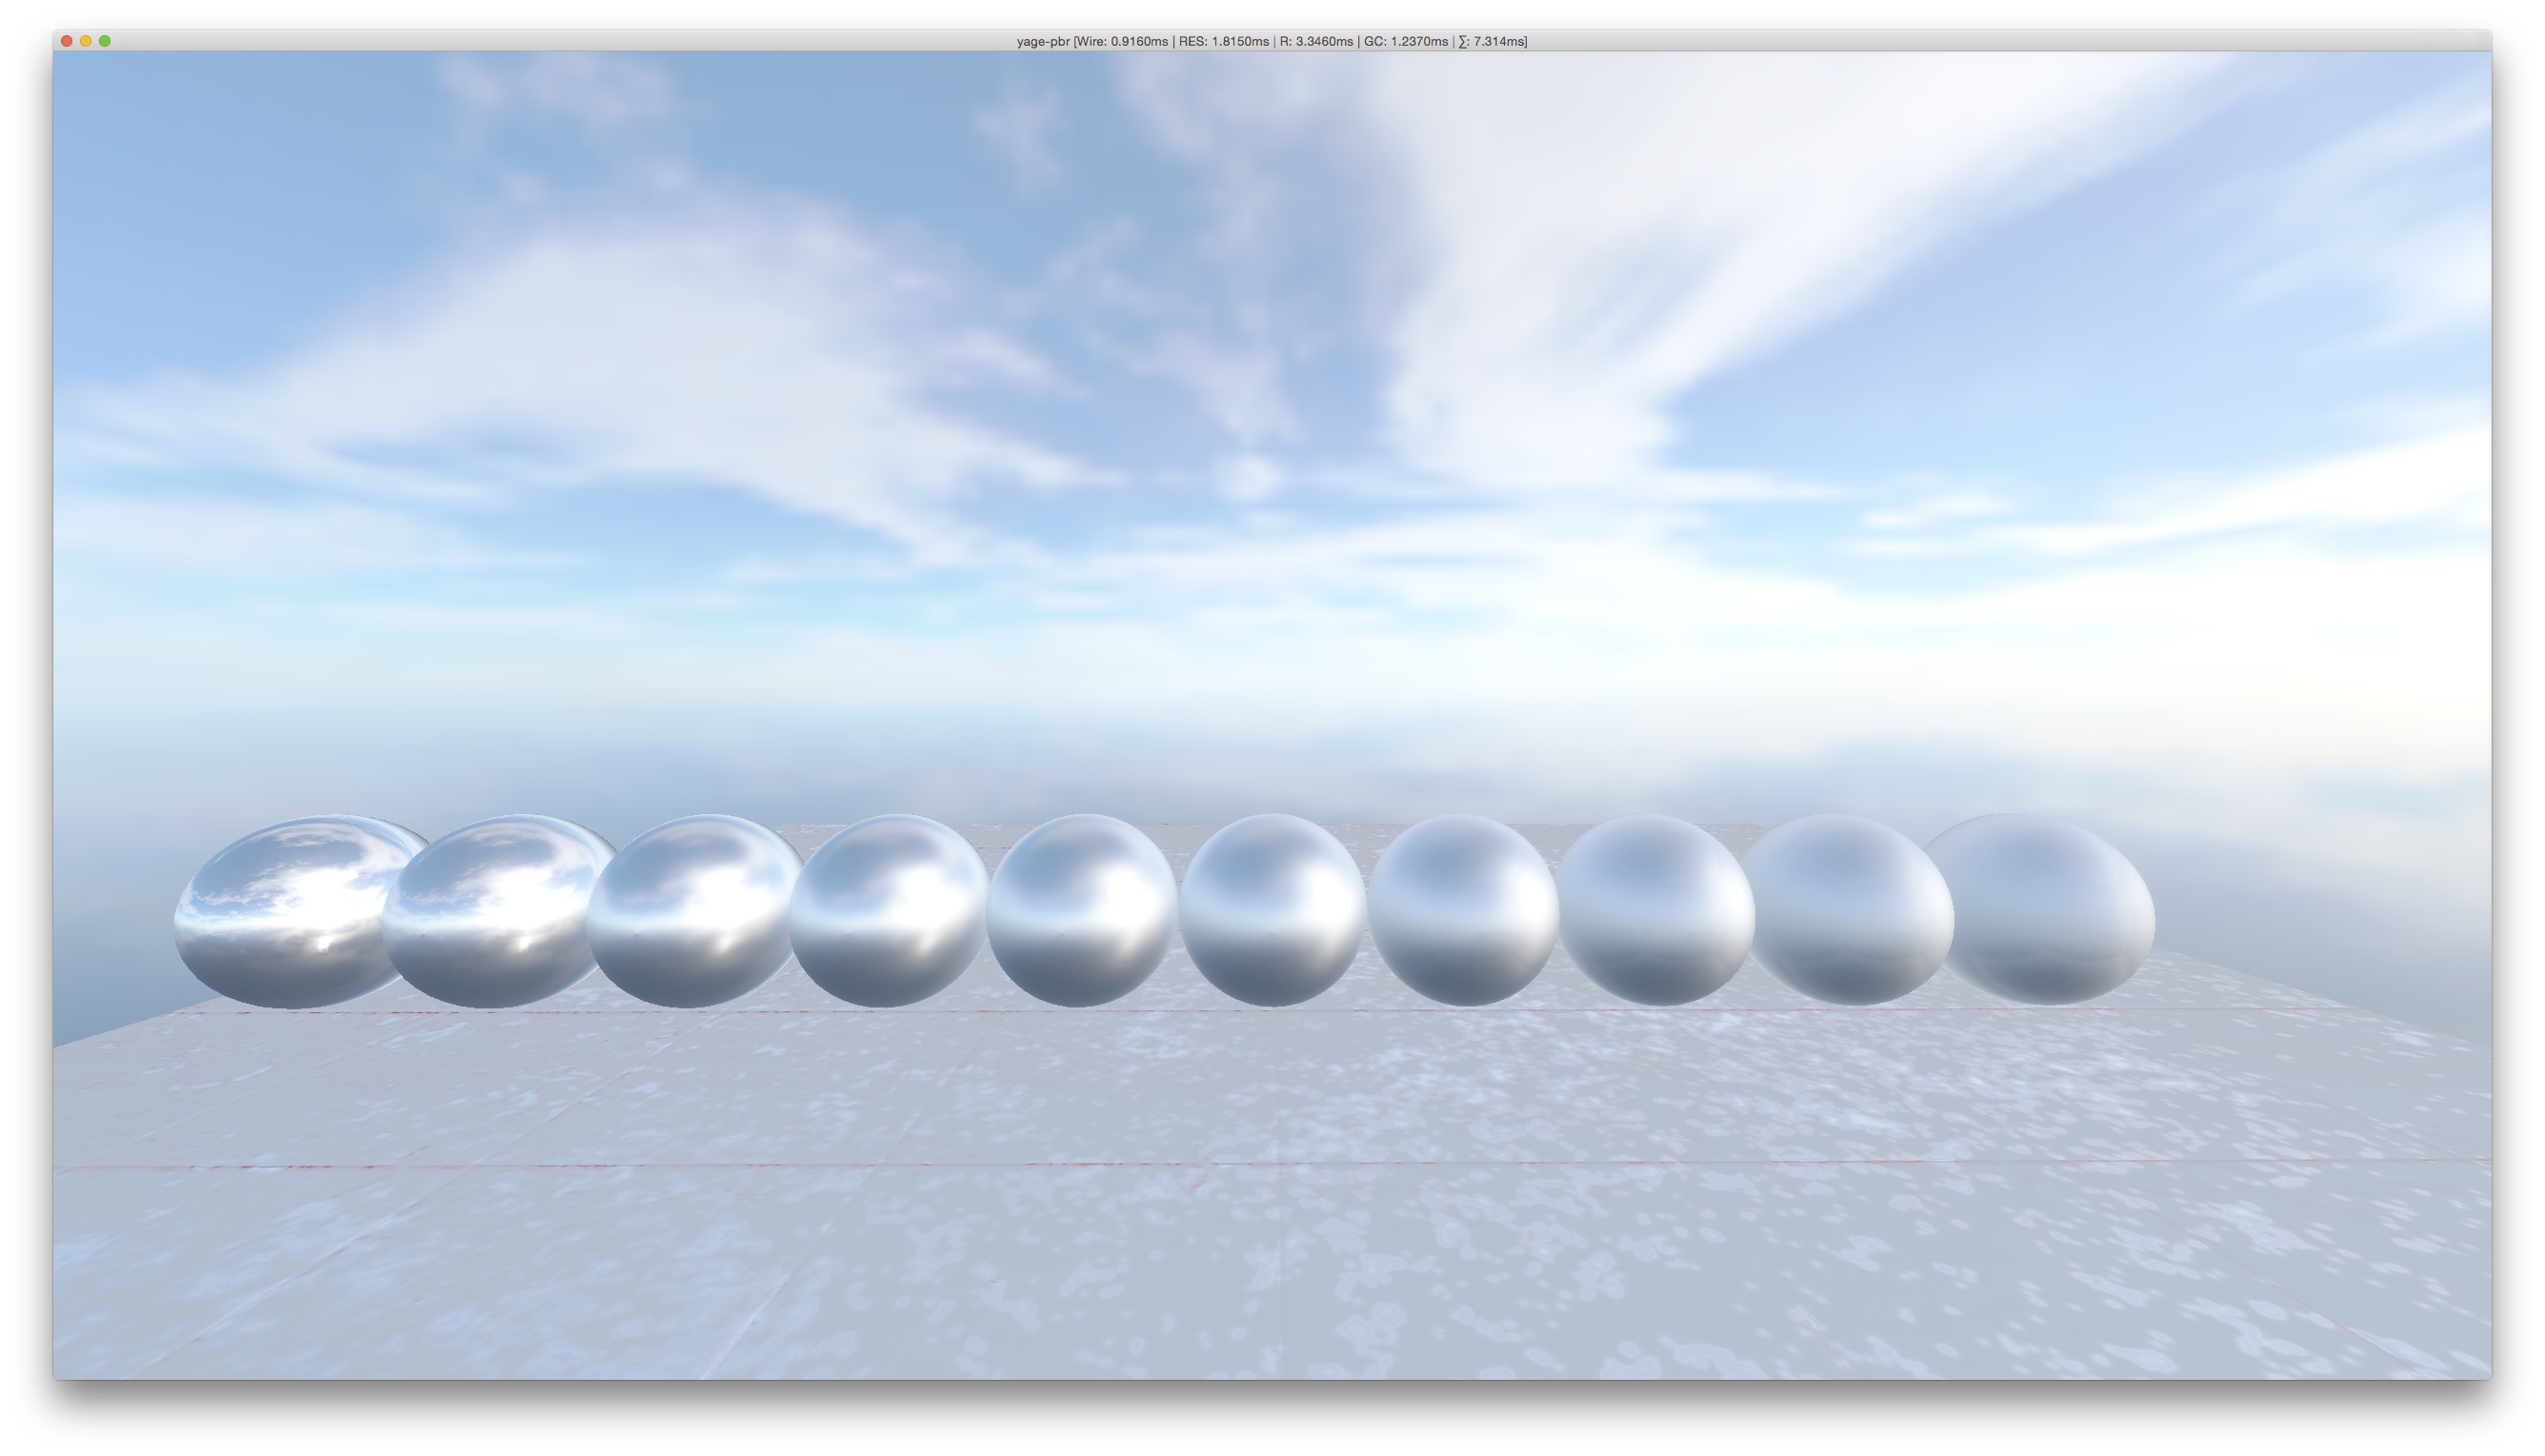
\includegraphics[width=.8\textwidth]{shots/pbr01}
\end{figure}

Da die entwickelte \ac{PBR} Pipeline zu umfangreich für eine umfassende Betrachtung im Detail ist, wird in \fref{chap:anwendung} exemplarisch ein Renderschritt der Pipeline als Baustein implementiert. Einen zusätzlichen Überblick über das Gesamtsystem der praktischen Implementierung bietet \fref{sec:src-pipeline} im Appendix. Darüber hinaus ist das Gesamtprojekt zu dieser Arbeit als DVD im Appendix in \fref{chap:dvd} angefügt.

Die entwicklete \ac{PBR}-Pipeline wird in \fref{chap:resultat} sowohl auf ihr Echtzeitverhalten als auch grafische Qualität beurteilt. Zusätzlich werden die produktiven Gesichtspunkte, beispielsweise Flexibilität und Wartbarkeit, untersucht. Probleme und Herausforderungen, die sich während der praktischen Umsetzung aufgetan haben, werden ebenso benannt und eingeordnet.

Abgeschlossen wird der schriftliche Teil der Arbeit in \fref{chap:ausblick} mit einem Ausblick auf zukünftige Entwicklungsmöglichkeiten und Anwendungsbereiche der entwickelten Grafik-Engine.

